\documentclass[11pt]{article}
\usepackage[T1]{fontenc}
\usepackage{lmodern}
\usepackage[margin=1in]{geometry}
\usepackage{amsmath,amssymb,amsthm,mathtools}
\usepackage{microtype}
\usepackage{enumitem}
\usepackage{booktabs,tabularx,array}
\usepackage{caption}
\usepackage{tikz}
\usepackage{needspace}
\usepackage{xcolor}
\usepackage[numbers,sort&compress]{natbib}
\usepackage{hyperref}
\definecolor{inkblue}{RGB}{25,67,104}
\definecolor{softgray}{RGB}{103,113,122}
\hypersetup{
  colorlinks=true,linkcolor=inkblue,citecolor=inkblue,urlcolor=inkblue,
  pdftitle={Matching Gradient--Hessian Query Bounds via a Smooth Macro-Block Construction},
  pdfauthor={Colombo Team}
}
\captionsetup{font=small,labelfont=bf}
\setlength{\emergencystretch}{2em}
\setlength{\parskip}{0.15em}
\widowpenalty=10000
\clubpenalty=10000
\displaywidowpenalty=10000
\setlist{itemsep=0.25em,topsep=0.4em}
\allowdisplaybreaks[1]
\newtheorem{theorem}{Theorem}[section]
\newtheorem{lemma}[theorem]{Lemma}
\newtheorem{proposition}[theorem]{Proposition}
\newtheorem{corollary}[theorem]{Corollary}
\theoremstyle{definition}
\newtheorem{definition}[theorem]{Definition}
\theoremstyle{remark}
\newtheorem{remark}[theorem]{Remark}
\newcommand{\R}{\mathbb R}
\newcommand{\E}{\mathbb E}
\newcommand{\PP}{\mathbb P}
\newcommand{\eps}{\varepsilon}
\newcommand{\norm}[1]{\left\|#1\right\|}
\newcommand{\ip}[2]{\left\langle#1,#2\right\rangle}
\newcommand{\op}{\mathrm{op}}
\newcommand{\Lip}{\operatorname{Lip}}
\newcommand{\diag}{\operatorname{diag}}
\newcommand{\Qrand}{Q_{\mathrm{rand}}}
\newcommand{\Qdet}{Q_{\mathrm{det}}}
\newcommand{\Rate}{\mathcal R}
\newcolumntype{Y}{>{\raggedright\arraybackslash}X}
\title{\bfseries Matching Gradient--Hessian Query Bounds\\
via a Smooth Macro-Block Construction}
\author{Colombo Team\\[0.3em]
  \small\href{mailto:colombo.2026@outlook.com}{\texttt{colombo.2026@outlook.com}}}
\date{}
\begin{document}
\maketitle
\begin{abstract}
We study the cost of finding an $\eps$-stationary point when a
value--gradient query costs one and a full-Hessian query costs $\tau\ge1$.
For bounded-below objectives with initial gap, gradient Lipschitz constant,
and Hessian Lipschitz constant at most one, we give an explicit smooth
construction establishing the high-dimensional randomized lower bound
\[
 \Omega\!\left(\min\{\tau^{1/3}\eps^{-3/2},\,\eps^{-7/4}\}\right).
\]
Together with existing deterministic algorithms, this yields matching
bounds without logarithmic losses. The proof groups $m^2$ delayed
linear-system problems into each macro block: its objective-gap cost is
$O(m^2)$, whereas resolving it requires $\Omega(m^3)$ ordinary queries
unless a Hessian query discloses the block. A protected quadratic and a
ladder of hidden gates keep all future curvature exactly invisible while
preserving global smoothness and excluding premature stationary points.
A stopped transcript argument covers arbitrary adaptive randomized
queries and outputs that were never queried. The only imported
information-theoretic ingredient is a delayed-disclosure matrix-vector
lower bound. The weighted rate also follows from an existing hierarchical
tradeoff construction; the present proof provides a separate,
globally $C^\infty$ realization with explicit analytic and oracle accounting.
\end{abstract}

\noindent\textbf{Keywords.}
Nonconvex optimization; oracle complexity; gradient--Hessian queries;
randomized lower bounds; Lipschitz Hessian.
\par\medskip
\begin{samepage}
\noindent\textbf{AI Usage.}
Nearly the entire research pipeline for this paper was carried out by
Colombo, powered by GPT-5.6 Sol.
\par
\end{samepage}

\section{Introduction}\label{sec:introduction}
How much should an optimization algorithm pay for curvature information?
When the objective has a Lipschitz Hessian, second-order methods can reduce
the number of iterations needed to find a point with a small gradient.
Their advantage depends, however, on the relative cost of obtaining a
Hessian. A query model with separate prices makes this dependence precise:
an ordinary query returns a function value and gradient at cost one, a
rich query returns the full second-order information at cost $\tau$, and
the total cost is $G+\tau H$.

We consider objectives on the entire Euclidean space under simultaneous
gradient and Hessian Lipschitz bounds. With the initial gap and both
smoothness constants normalized to one, define
\begin{equation}\label{eq:rate-intro}
 \Rate(\tau,\eps)
 :=\eps^{-3/2}\min\{\tau^{1/3},\eps^{-1/4}\}
 =\min\{\tau^{1/3}\eps^{-3/2},\eps^{-7/4}\}.
\end{equation}
The two terms describe a change in the useful role of Hessian queries.
For $1\le\tau\le\eps^{-3/4}$, the optimal cost scales as
$\tau^{1/3}\eps^{-3/2}$. Above this price, a gradient-only method attains
the optimal order $\eps^{-7/4}$. Our main theorem proves this statement
for randomized algorithms in a sufficient high-dimensional regime and
gives an explicit function family that realizes the lower bound.

\subsection{Related work and the role of this proof}
Cubic regularization established the basic second-order approach to
nonconvex stationarity \cite{nesterovpolyak}. Reusing Hessians reduces their
amortized cost: Doikov, Chayti, and Jaggi \cite{doikov} analyzed lazy
updates, Adil et al.\ \cite{adil} obtained the cube-root price dependence
up to logarithmic factors, and Chen et al.\ \cite[Theorem 4.1]{chen}
removed those factors. The last result yields the deterministic weighted
upper bound $O(\tau+\tau^{1/3}\eps^{-3/2})$. Independently of the Hessian
price, the restarted accelerated-gradient method of Li and Lin
\cite[Theorem 1]{lilin} gives the log-free bound $O(\eps^{-7/4})$.
These are the algorithmic inputs used here.

On the lower-bound side, Zhang et al.\ \cite[Theorem 3.1]{zhang} and
Zhou, Sugiyama, and Suzuki \cite[Theorem 6.1, $p=2$]{zhou} establish the
high-dimensional randomized first-order exponent $7/4$. The latter
work also proves the delayed-input matrix-vector theorem used in our
construction. A first-order lower bound by itself does not settle the
weighted problem: a full Hessian can reveal an entire hidden matrix at
once, even if learning that matrix through vector products is expensive.

Wu et al.\ \cite{wu} prove a separate-budget gradient--Hessian tradeoff.
Their quantitative construction also implies the weighted rate
\eqref{eq:rate-intro}, with a smaller sufficient dimension; Appendix~\ref{app:comparison}
records the scaling. Our contribution is an alternative construction
and proof. Table~\ref{tab:literature}
distinguishes the available guarantees.

\begin{table}[t]
\centering
\small
\setlength{\tabcolsep}{5pt}
\renewcommand{\arraystretch}{1.18}
\caption{Comparable guarantees in normalized units, for sufficiently
small $\eps>0$ and $\tau\ge1$.
$T=\eps^{-3/2}$ and $\Rate=\Rate(\tau,\eps)$.
All rows target $\norm{\nabla f}\le\eps$; bounds with $\widetilde O$
may hide logarithmic factors. First-order lower bounds restrict $H=0$.
The last two rows allow both query types and match the combined upper
bound. Dimension conditions apply to lower bounds.}
\label{tab:literature}
\begin{tabularx}{\textwidth}{@{}p{0.25\textwidth}p{0.29\textwidth}Y@{}}
\toprule
Work & Oracle and guarantee & Rate and applicable scope\\
\midrule
Li--Lin \cite{lilin}
& Deterministic, gradients only
& $O(\eps^{-7/4})$; all dimensions.\\
Adil et al.\ \cite{adil}
& Deterministic, mixed-query upper bound
& $\widetilde O(\tau+\tau^{1/3}T)$; use the gradient-only bound when cheaper.\\
Chen et al.\ \cite{chen}
& Deterministic, mixed-query upper bound
& $O(\tau+\tau^{1/3}T)$; together with Li--Lin, $O(\Rate)$.\\
Zhang et al.\ \cite{zhang}; Zhou et al.\ \cite{zhou}
& Randomized, value--gradient lower bound
& $\Omega(\eps^{-7/4})$; sufficiently high dimension, $H=0$.\\
\midrule
Wu et al.\ \cite{wu}, construction consequence
& Randomized, mixed-query lower bound
& $\Omega(\Rate)$; $d\ge C[\min\{\tau,\eps^{-3/4}\}+\log(2+T)]$. See Appendix~\ref{app:comparison}.\\
This paper, Theorem~\ref{thm:main}
& Randomized lower bound from independent delayed systems
& $\Omega(\Rate)$; dimension \eqref{eq:dimension-main}; globally $C^\infty$ hard instances.\\
\bottomrule
\end{tabularx}
\end{table}

\paragraph{Proof ingredients and attribution.}
The proof uses the one-phase linear-system result of Zhou et al.\
\cite[Lemma 6.9]{zhou}. Its localized gates and positive clipped forcings
also build on their chain construction; we give all analytic estimates
needed here. The mixed-query argument adds three components: a macro
quadratic whose curvature is hidden until admission; a stationary-energy
estimate that controls its signed boundary contribution; and an
increasing-radius gate chain that transmits admission at bounded
third-derivative cost. A disclosure calendar then converts these analytic
properties into a weighted lower bound.

\paragraph{Organization.}
Section~\ref{sec:model} states the model and theorem and derives the upper
bound from existing algorithms. Section~\ref{sec:overview} explains the
scales behind the lower bound. Sections~\ref{sec:input}--\ref{sec:stationarity}
give the external input, the explicit scalar construction, and the
stationarity argument. Section~\ref{sec:information} proves the mixed-oracle
resource inequality, and Section~\ref{sec:calibration} completes the
normalization. Section~\ref{sec:consequences} discusses consequences and scope.

\section{Oracle model and main theorem}\label{sec:model}
\subsection{Function class and query costs}
Let $\mathcal F_d$ be the class of bounded-below $C^2$ functions
$f:\R^d\to\R$ such that, with initial point zero,
\begin{equation}\label{eq:class}
 f(0)-\inf f\le1,\qquad
 \Lip(\nabla f)\le1,\qquad
 \Lip(\nabla^2 f)\le1.
\end{equation}
Vector norms are Euclidean, and matrix norms are operator norms.
We use the following exact oracles:
\[
 \mathsf O_1(x)=(f(x),\nabla f(x)),
 \qquad
 \mathsf O_2(x)=(f(x),\nabla f(x),\nabla^2f(x)).
\]
An $\mathsf O_1$ call costs one; an $\mathsf O_2$ call costs $\tau\ge1$.
If an execution uses $G$ ordinary calls and $H$ rich calls, its cost is
$G+\tau H$. Local computation is free. A separate value query, if used,
is charged as an ordinary call.

The query points, query types, stopping decisions, and final output may
be arbitrary Borel-measurable functions of the transcript and an
independent random seed. The output need not be a queried point.
An algorithm has budget $B$ if its cost is at most $B$ on every input
and every execution. In particular, the budget is a hard cap.

Define $\Qrand^{(d)}(\tau,\eps)$ as the infimum of such budgets over
algorithms satisfying
\[
 \PP\!\left(\norm{\nabla f(\widehat x)}\le\eps\right)\ge\frac23
 \qquad\text{for every }f\in\mathcal F_d.
\]
The deterministic analogue $\Qdet^{(d)}$ requires success on every input.
The lower bound allows both strengthened packets above.
The upper-bound methods also apply to gradient-only ordinary calls and
Hessian-only rich calls, with the ordinary queries counted explicitly below.

\begin{samepage}
\subsection{The weighted frontier}
\begin{theorem}[Matching weighted query bounds]\label{thm:main}
There are universal constants $c,C,C_d,\eps_0>0$ such that, for
$0<\eps\le\eps_0$, $\tau\ge1$, and
\begin{equation}\label{eq:dimension-main}
 d\ge
 \max\!\left\{
   \lceil\tau\rceil,\,
   C_d\eps^{-9/2}\min\{\tau^{2/3},\eps^{-1/2}\}
 \right\},
\end{equation}
the complexities satisfy
\begin{equation}\label{eq:main}
 c\Rate(\tau,\eps)
 \le \Qrand^{(d)}(\tau,\eps)
 \le \Qdet^{(d)}(\tau,\eps)
 \le C\Rate(\tau,\eps).
\end{equation}
Equivalently, both randomized and deterministic complexities have order
\begin{equation}\label{eq:two-regimes}
 \begin{cases}
  \tau^{1/3}\eps^{-3/2},&1\le\tau\le\eps^{-3/4},\\[0.15em]
  \eps^{-7/4},&\tau\ge\eps^{-3/4}.
 \end{cases}
\end{equation}
The lower bound is witnessed by a distribution of globally $C^\infty$,
coercive functions sampled independently of the algorithm.
\end{theorem}
\end{samepage}

The sufficient dimension in \eqref{eq:dimension-main} records the cost of
the product construction proved below. It is not necessary for the rate,
as the comparison in Appendix~\ref{app:comparison} shows, and it gives no
fixed-dimensional conclusion. The upper bound itself is dimension-free.

\begin{figure}[htbp]
\centering
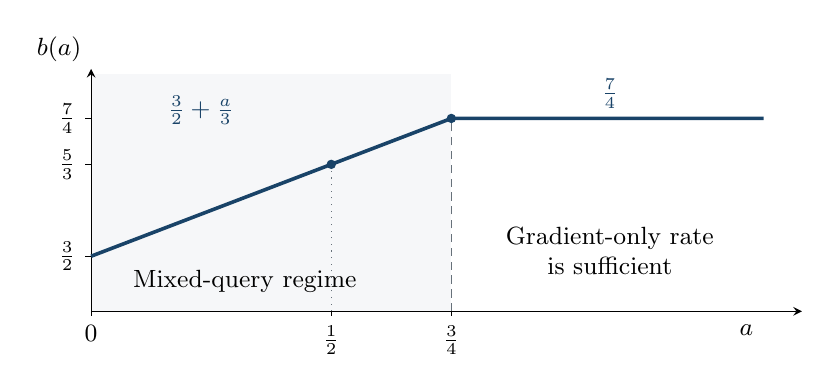
\begin{tikzpicture}[x=6.1cm,y=7cm,>=stealth,font=\small]
  \fill[inkblue!4] (0,0) rectangle (.75,.43);
  \draw[->] (0,0)--(1.48,0);
  \draw[->] (0,0)--(0,.44);
  \draw[softgray,densely dashed] (.75,0)--(.75,.35);
  \draw[softgray,dotted] (.5,0)--(.5,.266667);
  \draw[inkblue,line width=1.3pt] (0,.1)--(.75,.35)--(1.4,.35);
  \fill[inkblue] (.5,.266667) circle (1.7pt);
  \fill[inkblue] (.75,.35) circle (1.7pt);
  \foreach \x/\label in {0/0,.5/{\tfrac12},.75/{\tfrac34}} {
    \draw (\x,0)--(\x,-.008);
    \node[below] at (\x,-.008) {$\label$};
  }
  \foreach \y/\label in {.1/{\tfrac32},.266667/{\tfrac53},.35/{\tfrac74}} {
    \draw (0,\y)--(-.012,\y);
    \node[left] at (-.012,\y) {$\label$};
  }
  \node[below right] at (1.33,-.006) {$a$};
  \node[above left] at (0,.435) {$b(a)$};
  \node[inkblue,anchor=west] at (.14,.365) {$\frac32+\frac a3$};
  \node[inkblue,above] at (1.08,.35) {$\frac74$};
  \node[align=center] at (.32,.055) {Mixed-query regime};
  \node[align=center] at (1.08,.11) {Gradient-only rate\\is sufficient};
\end{tikzpicture}
\caption{Accuracy exponent of the matched cost:
if $\tau=\eps^{-a}$, then $\Rate(\tau,\eps)=\eps^{-b(a)}$ with
$b(a)=\min\{3/2+a/3,7/4\}$. The point $a=1/2$ gives exponent $5/3$.
The figure concerns the high-dimensional regime of Theorem~\ref{thm:main};
the vertical axis displays exponents, not absolute query counts.}
\label{fig:frontier}
\end{figure}

\subsection{Deriving the upper bound}
\begin{proposition}[Upper bound from existing algorithms]\label{prop:upper}
For every dimension, $0<\eps\le\eps_0$, and $\tau\ge1$,
\[
 \Qdet^{(d)}(\tau,\eps)
 \le C\min\{\tau+\tau^{1/3}\eps^{-3/2},\,\eps^{-7/4}\}
 \le C'\Rate(\tau,\eps).
\]
\end{proposition}
\begin{proof}
Use the NALEN method of Chen et al.\ \cite[Theorem 4.1 and Algorithm 1]{chen}
with Hessian refresh period $m_H=\lceil\tau\rceil$.
It needs
$N=O(m_H+m_H^{1/3}\eps^{-3/2})$ iterations.
Including the gradients used to choose a certified output, at most
$3N+1$ ordinary calls and $\lceil N/m_H\rceil$ Hessian calls suffice.
Their weighted cost is bounded by
\[
 3N+1+\tau\lceil N/m_H\rceil\le4N+\tau+1.
\]
All subproblem computations use the returned data. An upper bound on
the initial gap can be used to select the parameters; a zero initial
gradient permits immediate termination.

Alternatively, Li and Lin's gradient-only method \cite[Theorem 1]{lilin}
uses $O(\eps^{-7/4})$ calls. Reducing its internal tolerance by the
universal output constant gives the requested gradient norm.
The possible final-epoch overhead is absorbed for $\eps\le\eps_0$.
For $\tau\le\eps^{-3/4}$, the initialization cost satisfies
$\tau\le\tau^{1/3}\eps^{-3/2}$. For larger $\tau$, use the
gradient-only method. This proves the result.
\end{proof}

\section{How the lower-bound scales fit together}\label{sec:overview}
The rate is determined by the work hidden in one macro block relative
to the objective gap needed to realize that block. Put $T=\eps^{-3/2}$.
For an integer $m$, each macro contains $k=m^2$ linear systems.
After its right-hand side is disclosed, one system requires
$r=\Theta(m)$ matrix-vector products before its solution can be
approximated. The $k$ systems are linked sequentially, so ordinary
queries must spend $s=kr=\Theta(m^3)$ calls on the macro. A rich query
is allowed to disclose the entire active macro.

\begin{table}[h]
\centering
\small
\renewcommand{\arraystretch}{1.18}
\caption{Scales in the product construction. The bounds are uniform in
the number of macros and in the dimension of each vector variable.}
\label{tab:scales}
\begin{tabularx}{\textwidth}{@{}p{0.43\textwidth}p{0.20\textwidth}Y@{}}
\toprule
Quantity & Scale & Role\\
\midrule
Micro systems per macro, $k$ & $m^2$ & Objective-gap cost per macro.\\
Post-disclosure delay, $r$ & $\Theta(m)$ & Hardness of one linear system.\\
Ordinary work per macro, $s=kr$ & $\Theta(m^3)$ & Cost that a rich query can bypass.\\
Number of macros, $n$ & $\Theta(T/m^2)$ & Fits the normalized initial gap.\\
$\sup\norm{\nabla^2F}$; $\sup\norm{D^3F}$ & $O(m^2)$; $O(1)$ & Enforces both smoothness constraints.\\
Allowed block size & $m\le\eps^{-1/4}$ & Ensures $m^2\sqrt\eps\le1$.\\
\bottomrule
\end{tabularx}
\end{table}

The resource argument proves a lower cost of
\begin{equation}\label{eq:overview-cost}
 n\min\{\tau,s\}
 \asymp
 \frac{T}{m^2}\min\{\tau,m^3\}.
\end{equation}
Choosing $m$ of order
$\min\{\tau^{1/3},\eps^{-1/4}\}$ gives \eqref{eq:rate-intro}.
Integer rounding and bounded prices are handled in
Section~\ref{sec:calibration}.

Three analytic requirements make this counting argument valid for a
single function on all of $\R^d$. First, an unadmitted macro must
contribute no hidden curvature to any derivative channel. Second,
clipping its quadratic outside a bounded region must not create a
stationary point from which the algorithm could stop early. Third, the
gate that hides a macro must have a large enough radius to absorb the
derivatives of its quadratic, without incurring an excessive objective
gap. The protected quadratic and the radius ladder address these
requirements. The subsequent simulation proves that the required gate
locations remain unknown under arbitrary adaptive exact-real queries.

\section{Delayed-disclosure linear-system hardness}\label{sec:input}
The information-theoretic input is a linear-system problem in which
the matrix can be queried before its right-hand side is known.
Such early products do not eliminate the need for a subsequent sequence
of products in a fresh direction. We use the following specialization of
Zhou et al.\ \cite[Lemma 6.9]{zhou}, with internal accuracy and smallest
eigenvalue both equal to one.

\begin{samepage}
\begin{lemma}[Delayed-input matrix-vector hardness; external input]\label{lem:external}
There are constants $c_0,C_0,\kappa_0>0$. Let $k\ge\kappa_0$, $r=\lfloor c_0\sqrt{k}\rfloor\ge1$, and integers $Q\ge r$ and $L\ge1$. For $\delta\in(0,1/4)$ and
\begin{equation}\label{eq:M}
 M\ge C_0\left(Q^2+k\left[Q+\log\frac{(Q+2)L}{\delta}\right]\right),
\end{equation}
there is an algorithm-independent law of $(A,b)\in\R^{M\times M}\times\R^M$ supported on
\begin{equation}\label{eq:phase-data}
 I\preceq A\preceq kI,\qquad \norm b=B_*=512,\qquad
 16\le\norm{A^{-1}b}\le B_*.
\end{equation}
A procedure may obtain at most $Q$ adaptive products with $A$ before receiving $b$, and fewer than $r$ products afterward. With at most $L$ recorded candidate vectors, including pre-disclosure candidates and unqueried outputs, the probability that any candidate has distance strictly less than $3$ from $A^{-1}b$ is at most $\delta$. The disclosure time may be chosen adaptively using only the pre-disclosure transcript. Queries and candidates may be arbitrary Borel-measurable functions of the data available when they are selected.
\end{lemma}
\end{samepage}
We decrease $c_0$ if necessary so that $c_0\le1$. The cited law uses a Haar-rotated replicated spectrum and conditions on the norm event in \eqref{eq:phase-data}. That norm event has probability at least $7/8$ in the construction. These facts identify a fixed input law, rather than a resisting oracle chosen after observing the algorithm. In the cited notation the specialization is $\mu=\rho=\varepsilon_{\rm lin}=1$, $\bar L=k$, and $\kappa=k$; the $L_1$ used to name the spectral endpoint in that paper is $2k$. For the mixed-query application, fix the same law with $Q=ns+1$, $L=ns+2$, and $\delta=(12nk)^{-1}$ before choosing the optimization algorithm. The statement is thus not an algorithm-dependent distributional assertion.

\begin{remark}[Independent side data and stopping]\label{rem:stopping}
Independent side data may be fixed in applying Lemma~\ref{lem:external}. It also applies to candidates recorded before a stopping time at which the entire pair is disclosed: stop before that disclosure. If the stopping candidate precedes the $r$th post-disclosure product, record it and stop before requesting that product. If $b$ has not yet been supplied, pad with dummy products and disclose $b$ only after recording all candidates. These operations preserve the candidate list and meet the lemma's product budget. They do not condition the target law on the event that a particular stopping decision was made.
\end{remark}

\section{Smooth gates, positive forcings, and a protected quadratic}
\label{sec:primitives}
We now prepare three scalar components. A flat gate hides information
outside a target ball; a bounded positive forcing drives the next
variable once its predecessor is completed; and a public radial guard
prevents quadratic clipping from introducing spurious stationary points.
\subsection{Flat gates and bounded positive forcings}
All profiles in this section are fixed once and for all. All constants depending on them are universal. For an explicit choice, let
\[
 b_0(u)=\begin{cases}e^{-1/u},&u>0,\\0,&u\le0,\end{cases}
 \qquad S(u)=\frac{b_0(u)}{b_0(u)+b_0(1-u)}.
\]
Then $S$ is smooth and nondecreasing, with $S=0$ on $(-\infty,0]$ and $S=1$ on $[1,\infty)$. The profiles below may be taken as
$\eta(u)=1-S((u-4)/5)$, $\chi(u)=1-S(u-1)$,
$\zeta(u)=1-S(u-2)$, and $h(u)=S(u-1)$.

Choose smooth nonincreasing $\eta:[0,\infty)\to[0,1]$ with
\[
 \eta(u)=1\ (u\le4),\qquad \eta(u)=0\ (u\ge9).
\]
For a center $a$ and radius parameter $\rho$, set
\begin{equation}\label{eq:gate}
 \mathcal G_{a,\rho}(x)=\eta\!\left(\frac{\norm{x-a}^2}{\rho^2}\right).
\end{equation}
The gate, together with all its derivatives, vanishes when $\norm{x-a}\ge3\rho$. Its derivatives of order $j\le3$ have norm at most $C\rho^{-j}$, uniformly in dimension. Also
\begin{equation}\label{eq:gate-sign}
 \nabla\mathcal G_{a,\rho}(x)=-\alpha(x)(x-a),\qquad \alpha(x)\ge0.
\end{equation}

Choose a smooth nonincreasing $\chi:[0,\infty)\to[0,1]$ equal to one on $[0,1]$ and zero on $[2,\infty)$. Write
$\pi_R(x)=\chi(\norm x/R)x$ and let $a_\chi$ bound $\norm{D\pi_R}$ for every $R$. Fix
\[
 R_0>(a_\chi+2)B_*+10,\qquad H_0=4B_*R_0.
\]
For $\norm b=B_*$ and $\rho\ge1$, define the positive bounded forcing
\begin{equation}\label{eq:forcing}
 \Phi_{b,\rho}(x)=H_0\rho+\ip b{\pi_{R_0\rho}(x)}.
\end{equation}
It satisfies
\begin{equation}\label{eq:forcing-bounds}
 c\rho\le\Phi_{b,\rho}\le C\rho,\quad
 \norm{\nabla\Phi_{b,\rho}}\le C,\quad
 \norm{\nabla^2\Phi_{b,\rho}}\le C/\rho,\quad
 \norm{D^3\Phi_{b,\rho}}\le C/\rho^2.
\end{equation}
It is exactly $H_0\rho+\ip b x$ on $\norm x\le R_0\rho$.

\subsection{The public radial guard}
The quadratic to be hidden has curvature of order $k$.
Clipping it at radius of order $k$ keeps its third derivative bounded,
but the clipping derivative may point inward. The following public
radial term compensates for that derivative uniformly over the hidden
matrix and the admission multiplier.
Let $B$ be any positive semidefinite matrix with $\norm B\le k$. Set $R=C_Rk$, where $C_R$ will be fixed below independently of $k$. Choose smooth profiles $\zeta,h$ such that
\[
 \zeta=1\text{ on }[0,2],\quad\zeta=0\text{ on }[3,\infty),\quad
 0\le\zeta\le1,\quad\zeta'\le0,
\]
\[
 h=0\text{ on }[0,1],\quad h=1\text{ on }[2,\infty),\quad
 0\le h\le1,\quad h'\ge0.
\]
Put $\psi(s)=\int_0^s u h(u)\,du$ and define
\begin{equation}\label{eq:cap-guard}
 Q_B(z)=\frac12z^TBz,\quad
 \overline Q_B(z)=\zeta(\norm z/R)Q_B(z),\quad
 P_k(z)=\frac12\norm z^2+KkR^2\psi(\norm z/R).
\end{equation}
Here $K$ is a sufficiently large fixed constant depending only on $\zeta$.

\begin{lemma}[Protected quadratic]\label{lem:guard}
For $0\le t\le1$ and every $z$,
\begin{equation}\label{eq:radial-guard}
 \ip z{\nabla P_k(z)+t\nabla\overline Q_B(z)}\ge\norm z^2.
\end{equation}
Both $P_k$ and $\overline Q_B$ are nonnegative. On $\norm z\le R$, $P_k=\norm z^2/2$ and $\overline Q_B=Q_B$. Globally,
\begin{align}\label{eq:cap-bounds}
 |\overline Q_B|&\le Ck^3,&
 \norm{\nabla\overline Q_B}&\le Ck^2,&
 \norm{\nabla^2\overline Q_B}&\le Ck,&
 \norm{D^3\overline Q_B}&\le C,\\
 \norm{\nabla^2P_k}&\le Ck,&
 \norm{D^3P_k}&\le C.&&&&\nonumber
\end{align}
The constants are independent of the dimension.
\end{lemma}
\begin{proof}
For $s=\norm z/R$, homogeneity gives
\[
 \ip z{\nabla\overline Q_B(z)}=(2\zeta(s)+s\zeta'(s))Q_B(z).
\]
It is nonnegative for $s\le2$ and zero for $s\ge3$. In the transition annulus it is at least $-Ck\norm z^2$. The extra public radial derivative equals $Kk\norm z^2h(s)$, and $h=1$ throughout that annulus. Choosing $K\ge C$ proves \eqref{eq:radial-guard}. The derivative estimates follow by differentiating the radial profiles on annuli bounded away from zero: each differentiation costs $R^{-1}$, and the quadratic scale is $kR^2$. Since $R=C_Rk$, the third-derivative scale is $k/R=O(1)$. The guard is identically zero near zero and quadratic outside a fixed annulus, so there is no singularity from the Euclidean norm at zero.
\end{proof}

\section{The smooth macro-block objective}\label{sec:construction}
For a positive integer $k$, write $[k]=\{1,\ldots,k\}$.
Fix an integer $m\ge m_0$, where $m_0$ is an integer satisfying
\[
 m_0\ge\max\{2,\sqrt{\kappa_0},2/c_0\},
\]
and put
\[
 k=m^2,\qquad r=\lfloor c_0m\rfloor,\qquad s=kr.
\]
In particular, $(c_0/2)m\le r\le m$, and $(c_0/2)m^3\le s\le m^3$.
Choose $n$ macro blocks. Each contains $k$ micro variables $z_{i,1},\ldots,z_{i,k}\in\R^M$. Independently draw $(A_{i,j},b_{i,j})$ from Lemma~\ref{lem:external}, and set
\[
 a_{i,j}=A_{i,j}^{-1}b_{i,j},\quad
 G_{i,j}=\mathcal G_{a_{i,j},1},\quad
 \Phi_{i,j}=\Phi_{b_{i,j},1},\quad
 B_i=\diag(A_{i,1}-I,\ldots,A_{i,k}-I).
\]
Write $z_i=(z_{i,1},\ldots,z_{i,k})$. Notice that $0\preceq B_i\preceq kI$.

\subsection{Increasing gate radii}
A radius-one gate can reveal the next micro forcing at bounded
derivative cost. Hiding a whole macro quadratic requires a gate of
radius $k$. We connect these two scales by auxiliary variables, called
amplifiers, whose radii grow along a short ladder.
Set $\rho_1=2$ and repeatedly set
\[
 \rho_{\ell+1}=\min\{\rho_\ell^2,k\}
\]
until the last value $\rho_J=k$ is reached. Thus
\begin{equation}\label{eq:ladder}
 J=O(1+\log\log(k+2)),\qquad
 \rho_{\ell+1}\le\rho_\ell^2,\qquad
 \sum_{\ell=1}^J\rho_\ell\le Ck.
\end{equation}
For each macro $i$, introduce $y_{i,\ell}\in\R^M$, independent uniform vectors $u_{i,\ell}$ on the unit sphere, and
\[
 c_{i,\ell}=B_*u_{i,\ell},\qquad
 a^{\rm amp}_{i,\ell}=\rho_\ell c_{i,\ell},\qquad
 g_{i,\ell}=\mathcal G_{a^{\rm amp}_{i,\ell},\rho_\ell},\qquad
 \phi_{i,\ell}=\Phi_{c_{i,\ell},\rho_\ell}.
\]
The public quadratic of this variable is $\norm{y_{i,\ell}}^2/(2\rho_\ell)$.
Define the macro admission multipliers
\[
 t_1=1,\qquad t_i=g_{i-1,J}(y_{i-1,J})\quad (i\ge2).
\]

\subsection{The scalar objective}
For a universal constant $D_*>0$, chosen after the energy estimate in Lemma~\ref{lem:energy}, let
\begin{equation}\label{eq:Psi}
 \Psi_i(z_i)=D_*k+\Phi_{i,1}(z_{i,1})
       +\sum_{j=1}^{k-1}G_{i,j}(z_{i,j})\Phi_{i,j+1}(z_{i,j+1}).
\end{equation}
On the product of all micro and amplifier coordinates, define
\begin{align}\label{eq:objective}
 F(z,y)={}&\sum_{i=1}^n
 \left[P_k(z_i)+t_i\big(\overline Q_{B_i}(z_i)-\Psi_i(z_i)\big)\right]\\
 &+\sum_{i=1}^n\sum_{\ell=1}^J\frac{\norm{y_{i,\ell}}^2}{2\rho_\ell}
 -\sum_{i=1}^nG_{i,k}(z_{i,k})\phi_{i,1}(y_{i,1})\nonumber\\
 &-\sum_{i=1}^n\sum_{\ell=1}^{J-1}
       g_{i,\ell}(y_{i,\ell})\phi_{i,\ell+1}(y_{i,\ell+1}).\nonumber
\end{align}
The three types of coupling in \eqref{eq:objective} have distinct roles.
The multiplier $t_i$ admits the quadratic and micro chain of macro $i$.
The terminal micro gate starts its amplifier chain, and the last amplifier
admits macro $i+1$. The terminal micro-to-amplifier link has no factor
$t_i$. Its derivative is bounded separately in Lemma~\ref{lem:energy},
and the information argument explicitly accounts for premature hits
of this gate.

\begin{lemma}[Gap and uniform smoothness]\label{lem:smooth}
With universal constants fixed as below, every realization of \eqref{eq:objective} is $C^\infty$, coercive, and satisfies
\begin{equation}\label{eq:regularity}
 F(0)-\inf F\le C_gnk,\qquad
 \sup_x\norm{\nabla^2F(x)}\le C_1k,\qquad
 \sup_x\norm{D^3F(x)}\le C_2.
\end{equation}
\end{lemma}
\begin{proof}
All negative terms are bounded, and every clipped quadratic
$\overline Q_{B_i}$ is nonnegative. Equations
\eqref{eq:forcing-bounds} and \eqref{eq:ladder} give the explicit lower bound
\[
 F(z,y)\ge\frac{\norm{(z,y)}^2}{2k}-C_gnk.
\]
This proves coercivity. At zero, every micro and amplifier gate vanishes
because its center is farther away than three gate radii. Thus
$F(0)=-(D_*k+H_0)\le0$, which also gives the initial-gap estimate.

Write $\Psi_i=D_*k+L_i$. Bounded overlap of the one-block and adjacent-block terms gives
\begin{equation}\label{eq:Psider}
 0\le L_i\le Ck,\quad \norm{\nabla L_i}\le C\sqrt k,\quad
 \norm{\nabla^2L_i}\le C,\quad \norm{D^3L_i}\le C.
\end{equation}
For completeness, color the adjacent-block edges with two colors. Terms of one color have disjoint supports. For third derivatives on disjoint supports $P_j$,
\[
 \sum_j\norm{P_ju}\norm{P_jv}\norm{P_jw}
 \le\norm u\norm v\norm w;
\]
the analogous Hessian estimate is Cauchy--Schwarz. Only a constant number of color classes is used.

For $i\ge2$, derivatives of $t_i$ of order $a\le3$ are $O(k^{-a})$, because the last amplifier radius is $k$. By \eqref{eq:cap-bounds}, the terms in the third derivative of $t_i\overline Q_{B_i}$ have respective scales
\[
 1,\qquad k^{-1}k,\qquad k^{-2}k^2,\qquad k^{-3}k^3.
\]
Every one is $O(1)$, and the corresponding Hessian terms are $O(k)$. Equations \eqref{eq:Psider} give the same or smaller bounds for $t_i\Psi_i$. The case $t_1=1$ is immediate.

An amplifier link from radius $\rho$ to radius $\rho'$ has third-derivative scales bounded by
\[
 C\left(\frac{\rho'}{\rho^3}+\frac1{\rho^2}
          +\frac1{\rho\rho'}+\frac1{(\rho')^2}\right),
\]
and Hessian scales bounded by
$C(\rho'/\rho^2+1/\rho+1/\rho')$.
They are uniformly bounded because $\rho'\le\rho^2$ and $\rho,\rho'\ge1$. The initial link has radii $1$ and $2$, so is also uniformly bounded.

Distinct macro terms in the first line of \eqref{eq:objective} have disjoint supports: each uses its own $z_i$ and the preceding last amplifier. Amplifier links can again be colored with a constant number of colors; the initial links also have disjoint supports. Add the public quadratics and use Lemma~\ref{lem:guard}. This proves the global estimates, without a factor depending on $n$, $k$, or $J$.
\end{proof}

\section{Stationarity forces completion of every block}\label{sec:stationarity}
To connect information acquisition with optimization, we must show
that every point with gradient norm at most one completes every gate.
The cross-macro term $t_i\overline Q_{B_i}$ requires special care:
its derivative in the preceding amplifier has the opposite sign from
the positive forcing. The following energy estimate bounds this
contribution at every nearly stationary point, uniformly as $t_i$
approaches zero.

\begin{lemma}[Stationary energy estimate]\label{lem:energy}
There are universal constants $C_R$ and $C_E$, independent of $D_*$, such that every point with $\norm{\nabla F}\le1$ satisfies, for every macro $i$,
\begin{equation}\label{eq:energy}
 \norm{z_i}\le C\sqrt k<R=C_Rk,
 \qquad \overline Q_{B_i}(z_i)=Q_{B_i}(z_i)\le C_Ek.
\end{equation}
In particular, choosing $D_*=C_E+1$ gives
\begin{equation}\label{eq:Wpositive}
 W_i(z_i):=\Psi_i(z_i)-\overline Q_{B_i}(z_i)\ge k>0
\end{equation}
at every such point.
\end{lemma}
\begin{proof}
Suppress $i$, and put $t=t_i$. Differentiating only with respect to $z_i$ gives
\[
 \nabla_{z_i}F=\nabla P_k(z)+t\nabla\overline Q_B(z)-tU(z)-V(z,y),
\]
where $U=\nabla L_i$, $\norm U\le C\sqrt k$, and
$V=\phi_{i,1}(y_{i,1})\nabla G_{i,k}(z_{i,k})$ is supported on the last micro block. Since $\rho_1=2$, $\norm V\le C$. These bounds do not involve $D_*$. Taking an inner product with $z$ and using \eqref{eq:radial-guard} gives
\[
 \norm z^2\le\norm z\big(1+C\sqrt k+C\big).
\]
Choose $C_R$ larger than the resulting universal coefficient. Then $\norm z<R$, so the public guard is inactive and the clipped quadratic equals the original quadratic, including its derivatives.

Let $e=\nabla_{z_i}F$, $\norm e\le1$. Therefore
\[
 (I+tB)z=tU+V+e.
\]
For every eigenvalue $\lambda\in[0,k]$ and $t\in[0,1]$,
\[
 \frac{t^2\lambda}{(1+t\lambda)^2}\le\frac{t}{4}\le\frac14,
 \qquad \frac{\lambda}{(1+t\lambda)^2}\le k.
\]
The first inequality also holds at $t=0$. Using
$\norm{a+b}^2\le2\norm a^2+2\norm b^2$ yields
\begin{align*}
 Q_B(z)&=\frac12\norm{B^{1/2}(I+tB)^{-1}(tU+V+e)}^2\\
 &\le\frac14\norm U^2+k\norm{V+e}^2\le C_Ek.
\end{align*}
Finally $L_i\ge0$, so $D_*=C_E+1$ proves \eqref{eq:Wpositive}.
This positivity is needed only at nearly stationary points; no global
sign condition on $W_i$ is assumed.
\end{proof}

\begin{lemma}[Stationarity forces all gates open]\label{lem:stationary}
Every point with $\norm{\nabla F}\le1$ satisfies
\begin{equation}\label{eq:complete}
 \norm{z_{i,j}-a_{i,j}}\le1,\qquad
 \norm{y_{i,\ell}-a^{\rm amp}_{i,\ell}}\le\rho_\ell
\end{equation}
for every index. Hence all micro and amplifier gates equal one.
\end{lemma}
\begin{proof}
First establish that clipping in each forcing is inactive at a nearly stationary point. If a micro variable has norm greater than $R_0$, its outgoing gate is zero with all derivatives, since that gate is supported within norm $B_*+3<R_0$. Lemma~\ref{lem:energy} has already removed the macro cap and guard. The corresponding gradient is
$(I+t_i(A_{i,j}-I))z_{i,j}-t_i c\nabla\Phi_{i,j}$, with $0\le c\le1$. Its norm exceeds one by the definition of $R_0$. This is impossible. Thus every micro forcing is in its linear region.

For an amplifier at radius $\rho$, a norm greater than $R_0\rho$ likewise makes its own outgoing gate identically zero. Its gradient then equals $y/\rho-c\nabla\phi$, $c\in[0,1]$, and has norm greater than one. This argument also applies to the last amplifier, whose outgoing coefficient is the possibly signed function $W_{i+1}$: the gate derivative is zero there. Thus all amplifier forcings are linear at the point under consideration.

Proceed by induction. Macro one has $t_1=1$. If the incoming micro gate is one, its block gradient is
\[
 A_{i,j}(z_{i,j}-a_{i,j})-W\nabla G_{i,j}(z_{i,j})
  =(A_{i,j}+\alpha W I)(z_{i,j}-a_{i,j}),
\]
where $W=\Phi_{i,j+1}>0$ for $j<k$ and $W=\phi_{i,1}>0$ for $j=k$. By \eqref{eq:gate-sign}, $\alpha\ge0$. Since $A_{i,j}\succeq I$, a gradient norm at most one forces distance at most one, and therefore the outgoing gate is one. This proves all micro gates in the first macro are open.

At an amplifier with incoming gate one, the gradient similarly is
\[
 (\rho_\ell^{-1}I+\alpha W I)
        (y_{i,\ell}-a^{\rm amp}_{i,\ell}).
\]
For $\ell<J$, $W=\phi_{i,\ell+1}>0$. For $\ell=J$ and $i<n$, $W=W_{i+1}>0$ by Lemma~\ref{lem:energy}. For the final amplifier of the final macro, the outgoing coefficient is zero. In every case the distance is at most $\rho_\ell$, so its gate is one. In particular, the last amplifier makes $t_{i+1}=1$. Induct over the macros.
\end{proof}

The constants in the preceding lemmas are chosen before any instance
parameters. Appendix~\ref{app:constants} gives one explicit order of
selection and shows that the energy offset does not enter its own
defining estimate.


\section{From exact transcripts to a mixed-query lower bound}\label{sec:information}
We now relate the explicit scalar \eqref{eq:objective} to the weighted query cost.
The argument follows the information available in the exact transcript.
One ordinary call may supply products with every matrix of the active
macro, so counting matrix entries or coordinates would not suffice.

\begin{proposition}[Macro-block resource inequality]\label{prop:resource}
For every $n\ge1$, integer $m\ge m_0$, and sufficiently large $M$, the fixed distribution above has the following property. Let $s=kr$, and let an arbitrary randomized algorithm have a hard cap of $Q$ total calls, where $Q\le ns$, and suppose each of its executions satisfies
\begin{equation}\label{eq:joint-ineq}
 G+sH<ns.
\end{equation}
Then its average probability, over the fixed distribution, of outputting a point with gradient norm at most one is at most $1/6$. In particular, no algorithm with weighted budget
\begin{equation}\label{eq:block-cost}
 C_\tau<n\min\{\tau,s\}
\end{equation}
can succeed with probability $2/3$ on every realization.
One may take
\begin{equation}\label{eq:M-full}
 M=C\left((ns+1)^2+k\left[ns+1+
  \log\big((ns+3)^2nk\big)\right]
  +\log\big(n(J+1)(ns+2)\big)\right)
\end{equation}
rounded upward, with a sufficiently large universal $C$.
\end{proposition}

\subsection{True and masked experiments}
Fix a deterministic decision rule. We strengthen the oracle by giving
the algorithm additional products and scheduled disclosures of hidden
data. Original algorithms are included by ignoring these extra fields.
The \emph{true augmented experiment} always returns the actual derivative
packet of the sampled function, together with these additional fields.
The \emph{masked experiment} uses the same disclosure rules but suppresses
the gates specified below when forming its derivative packet.
We will prove equality of the two transcripts until a bad event.
The masked experiment is an auxiliary probability space; its replies
on other histories need not be realizable by a function.

Put $P=ns$. Enforce both the total-call cap and $G+sH<P$ on every history: before an action that would violate either cap, stop and output zero. This does not change any execution covered by the proposition's hypotheses. For the weighted corollary, also impose its weighted cap. These counters are used in both experiments, including on masked histories that might not be realizable by a genuine function.

All matrix--right-hand-side pairs and all amplifier directions are sampled in advance from the fixed product law. A state consists of an active macro $a$ and the number $q\in\{0,\ldots,s-1\}$ of ordinary calls charged to it. Every macro $i<a$ is fully disclosed. In macro $a$, exactly $j=\lfloor q/r\rfloor$ micro pairs are fully disclosed, and right-hand sides through $j+1$ are disclosed. No amplifier direction in macro $a$ or a future macro is disclosed. At initial admission set $a=1$, $q=0$, and disclose $b_{1,1}$.

\paragraph{Ordinary call.}
Freeze its point using the pre-reply history, and charge it to $a$. Obtain one product $A_{a,h}z_{a,h}$ for each $h\in[k]$, with all vectors fixed by this same point. Compute the masked value--gradient packet using the pre-reply disclosure state. Both experiments also return these products as ancillary fields. Then increase $q$ by one. If $q$ is a multiple of $r$, disclose the complete pair of phase $q/r$ and, unless $q=s$, the next right-hand side. If $q=s$, disclose the amplifier directions, retire macro $a$, and admit macro $a+1$ with its first right-hand side. No product with the newly admitted macro is requested on this call. Only the next candidate can use these new disclosures.
In particular, at the candidate preceding a phase's $r$th product
after right-hand-side disclosure, exactly $r-1$ such products have
been observed. The full pair becomes available only in the ensuing reply.

\paragraph{Hessian call.}
Freeze its point first. Disclose the complete data of the active macro, including every micro pair and every amplifier direction. The true experiment returns the genuine second-order packet.
In the masked experiment, the packet uses the newly disclosed
current-macro data, while the outgoing admission multiplier to macro
$a+1$, together with its derivatives, remains suppressed at this
frozen point. Retire macro $a$ and admit macro $a+1$ for subsequent candidates. This extra disclosure is permitted even when the actual query point is in a previously retired or inactive region; it only helps the augmented algorithm.

\paragraph{The masks.}
For an ordinary packet, evaluate disclosed micro gates literally and set all other micro gates identically to zero. Evaluate amplifier gates only in retired macros. The admission multiplier of every unadmitted macro is identically zero. Any product term with an identically zero factor is evaluated as zero without using the other factor's undisclosed data.
For a Hessian packet use the same prescription after revealing the current macro, except for the outgoing multiplier just specified. Thus all relevant derivatives of the current macro can be computed, while future quadratic data are not used. Retired data are evaluated exactly.

\subsection{Computing every disclosed scalar and derivative}
The only undisclosed data used by an ordinary packet in the active macro are its permitted matrix products and its already disclosed right-hand sides. To see this explicitly, let $B=B_a$, $z=z_a$, $u=\|z\|/R$, and $Q=\tfrac12z^TBz$. A single blockwise product determines $Bz$ and $Q$, and hence
\[
 \overline Q_B(z)=\zeta(u)Q,\qquad
 \nabla\overline Q_B(z)=\zeta(u)Bz+
 \frac{\zeta'(u)}{R\|z\|}Qz.
\]
The last expression is interpreted using the constant profile near zero. It also determines the derivative in the preceding key coordinate, namely $\overline Q_B(z)\nabla t_a$. A nonzero incoming micro forcing uses a right-hand side already disclosed by the calendar. The terminal micro-to-amplifier link is zero until the last micro pair is disclosed, which happens exactly when its whole macro retires.

For a full Hessian, all data in the current macro have just been provided. For the cross-macro term $t(y)W(z)$, every Hessian block is one of
\[
 t\nabla^2W,\qquad \nabla t\,\nabla W^T,
 \qquad \nabla W\,\nabla t^T,\qquad W\nabla^2t.
\]
All four blocks vanish when the incoming gate's two-jet vanishes. The same product rule applies to micro and amplifier links. This checks cross-coordinate Hessian blocks, not only diagonal matrix blocks. Exact function values are reconstructed from the same data and are never free extra observations.

\subsection{Premature hits and stopped simulations}
Every query point is a candidate recorded before its response; the terminal output is also a candidate. There are at most $P+1$ candidates, for which we use the convenient bound $P+2$. Define bad events in the \emph{unconditionally run masked experiment}:
\begin{enumerate}[label=(\roman*),leftmargin=*]
\item A candidate is in the open radius-$3$ ball of a micro target whose complete pair is unavailable before that candidate. In particular, the location of its full-disclosure Hessian call and the location preceding its $r$th post-right-hand-side product are included.
\item A candidate is in the open radius-$3\rho_\ell$ ball of an amplifier target whose macro is not yet retired before that candidate. This includes the frozen point of the Hessian call that retires the macro.
\end{enumerate}
No probability below is conditioned on absence of earlier bad events.

\begin{lemma}[Micro-gate probability]\label{lem:microprob}
For each micro phase, the probability of event (i) is at most $1/(12nk)$ under \eqref{eq:M-full}.
\end{lemma}
\begin{proof}
Fix all random data except the target pair. Independence of the product law leaves the target law unchanged. Simulate the masked experiment using a matrix-product oracle for this pair; all other answers are computable from the fixed side data. Prior to disclosure of its right-hand side, the target can be used only through the allowed products. The target right-hand side is requested at its calendar disclosure time, a decision measurable from the available transcript and the fixed side data.

Record target coordinates of every candidate before answering it. Stop after recording the earliest of: the candidate whose active-macro Hessian reply would disclose this pair; the candidate preceding this phase's $r$th post-right-hand-side product; or the algorithm's terminal output. Hessian calls in other macros do not cause this stopping rule. Do not request the prohibited product or inspect the full-disclosure reply. There are at most $P+1$ pre-disclosure products and fewer than $r$ post-disclosure products. All candidates counted by event (i) appear on this list. If the right-hand side has not been requested when the simulation stops, append dummy products and request it after recording the list.

This is a legal procedure for Lemma~\ref{lem:external} with $Q=P+1$, $L=P+2$, and $\delta=(12nk)^{-1}$. Equation~\eqref{eq:M-full} dominates its dimension requirement after enlarging its universal constant. Integrating over the independent side data proves the claim. In particular, the argument stops before a purchase, rather than conditioning the pair's distribution on the decision to purchase a Hessian.
\end{proof}

\begin{lemma}[Amplifier-gate probability]\label{lem:ampprob}
The total probability of event (ii) is at most $1/12$ under \eqref{eq:M-full} with sufficiently large constant.
\end{lemma}
\begin{proof}
Before a macro retires, none of its amplifier directions is used in the masked replies: the terminal micro gate feeding its first amplifier is still suppressed, all following amplifier gates are suppressed, and its outgoing gate is suppressed as well. Its public quadratics contain no hidden directions. Consequently the pre-candidate transcript, while this macro is unretired, is a function of variables independent of each such direction. This assertion is about the masked experiment and does not require conditioning on the good event.

For $u$ uniform on the unit sphere, $B_*=512$, and a fixed candidate $v$, the event $\|v-B_*\rho u\|<3\rho$ is empty at $v=0$. Otherwise it implies
\[
 \left\langle u,\frac{v}{\|v\|}\right\rangle
 >\frac{\|v\|^2+(B_*^2-9)\rho^2}{2B_*\rho\|v\|}
 \ge\sqrt{1-9/B_*^2}.
\]
The last inequality is AM--GM. For completeness, put $\theta=\sqrt{1-9/B_*^2}$ and write
$u=\xi/\norm{\xi}$ for a standard Gaussian vector $\xi$.
After rotating the fixed direction to the first coordinate and
conditioning on $S=\sum_{j=2}^M\xi_j^2$, the Gaussian tail bound gives
\[
 \PP(\ip u e\ge\theta)
 \le \frac12\E\exp\!\left(-\frac{\theta^2 S}{2(1-\theta^2)}\right)
 =\frac12(1-\theta^2)^{(M-1)/2}
 =\frac12\left(\frac3{B_*}\right)^{M-1}.
\]
This is at most $2e^{-cM}$, uniformly in the candidate and gate radius.
Apply the bound conditionally to each pre-candidate history and union
bound over at most $nJ(P+2)$ choices. The last logarithmic term in
\eqref{eq:M-full} makes the sum at most $1/12$. The estimate permits
arbitrarily large query locations.
\end{proof}

\begin{lemma}[Exact coupling before a bad event]\label{lem:coupling}
Using the same sampled input and decision rule, the true augmented and masked experiments have identical replies, actions, and calendars before the first bad candidate. If no bad event occurs through the terminal candidate, their outputs coincide.
\end{lemma}
\begin{proof}
Suppose their histories agree before a candidate. The decision rule fixes the same query type and location, or the same output. Outside its open support ball, an unavailable gate and all its derivatives vanish exactly. Therefore deleting that gate changes none of the value, gradient, or Hessian terms at a nonbad candidate. The product-rule blocks displayed above also rule out any hidden cross-coordinate channel.

For an ordinary reply, the derivative packet is computed before the calendar update, so a just-retired pair or admitted macro is not used retroactively. On a Hessian reply, the current macro is computed exactly using its newly disclosed data. Its last amplifier was unknown at candidate selection; outside its support ball its two-jet is zero, so suppressing the outgoing multiplier to the next macro changes nothing. Every future macro's unmasked terminal micro gate is covered by event (i). Thus the derivative packets agree at each nonbad queried candidate. The extra fields and updated calendars agree as well. Induction proves the claim; a terminal output needs no extra oracle query.
\end{proof}

\subsection{Resource accounting and randomized algorithms}
\begin{proof}[Proof of Proposition~\ref{prop:resource}]
By Lemmas~\ref{lem:microprob} and \ref{lem:ampprob}, the probability of any bad event is at most $1/6$. On its complement the exact coupling holds for the true augmented and masked experiments, including the terminal candidate. Retiring one macro requires either $s$ ordinary calls charged to it or one Hessian call. Calls are charged to only one active macro. Therefore retirement of all $n$ macros implies $G+sH\ge ns$.

If \eqref{eq:joint-ineq} holds, some macro is still active or unadmitted at output. In particular it has a micro phase not fully disclosed. Lemma~\ref{lem:stationary} says that a successful output lies within distance one of that phase's target. As a recorded candidate, this would be event (i), a contradiction on the good event. Success in the true augmented experiment is contained in the masked bad event. Its probability is thus at most $1/6$. Original algorithms are included by ignoring the augmentation fields.

For a weighted budget as in \eqref{eq:block-cost},
\[
 G+sH\le\max\{1,s/\tau\}(G+\tau H)<ns.
\]
Also the total number of calls is smaller than $ns$, since each call has price at least one. This proves the weighted claim.

Finally, the function distribution is independent of the algorithm and of its seed. The argument applies after fixing any seed of a hard-budget randomized algorithm. Integrating first over the fixed input distribution and then over the seed gives average success at most $1/6$. Hence some realization has success probability less than $2/3$. This proves the unrestricted randomized lower bound, not merely a deterministic or zero-respecting bound.
\end{proof}

\section{Scaling the construction and proving the main theorem}\label{sec:calibration}
We finish the proof of Theorem~\ref{thm:main}. Let $T=\eps^{-3/2}$ and fix
\[
 \beta\ge\max\{1,C_1,\sqrt{C_2}\}.
\]
For an admissible $m$, set $k=m^2$ and
\[
 n=\left\lfloor\frac{T}{2\beta C_g k}\right\rfloor.
\]
It suffices to choose
\[
 \eps_0\le\min\{1,(2m_0)^{-4},(4\beta C_g)^{-1}\}.
\]
Then $T/(2\beta C_gk)\ge2$ for every $m_0\le m\le\eps^{-1/4}$, so $n\ge T/(4\beta C_gk)\ge1$. Define
\begin{equation}\label{eq:scaling}
 f(x)=\beta\eps^{3/2}F\!\left(\frac{x}{\beta\sqrt\eps}\right).
\end{equation}
Then $\nabla f=\eps\nabla F$ at the corresponding point, and
\[
 f(0)-\inf f\le\beta\eps^{3/2}C_gnk\le1,
\]
\[
 \sup\norm{\nabla^2f}\le\frac{C_1}{\beta}k\sqrt\eps\le1,
 \qquad
 \Lip(\nabla^2f)\le\frac{C_2}{\beta^2}\le1.
\]
Thus every realization belongs to the original class, and an $\eps$-stationary point of $f$ corresponds exactly to a unit-stationary point of $F$.

Put $a=\min\{\tau^{1/3},\eps^{-1/4}\}$. If $a\ge2m_0$, take $m=\lfloor a\rfloor$. Then $m\ge a/2$, $s=m^2\lfloor c_0m\rfloor=\Theta(m^3)$, and $s\le m^3\le\tau$. Proposition~\ref{prop:resource} gives
\[
 \Qrand^{(d)}(\tau,\eps)\ge cns\ge c'\frac{T}{m^2}m^3
 \ge c''Ta.
\]
If $a<2m_0$, use the fixed choice $m=m_0$. For sufficiently small $\eps$, this case has bounded $\tau$. Since $\min\{\tau,s\}\ge1$ and $n=\Theta(T)$, Proposition~\ref{prop:resource} gives $\Omega(T)=\Omega(Ta)$. The constants are universal because $m_0$ is fixed. Together with the upper bound already proved, this establishes \eqref{eq:main}.

\paragraph{Dimension.}
There are $n(k+J)$ vector variables, each of dimension $M$. In the calibration above $nk=\Theta(T)$, $s=\Theta(m^3)$, $ns=\Theta(Tm)$, and $J=O(k)$. Equation~\eqref{eq:M-full} permits $M=O(T^2m^2)$: the other terms are smaller for sufficiently small $\eps$ and $m\le\eps^{-1/4}$. Therefore
\[
 d_0=n(k+J)M=O(T^3m^2)
 =O\!\left(\eps^{-9/2}\min\{\tau^{2/3},\eps^{-1/2}\}\right).
\]
The bounded-$a$ case is absorbed into the same universal constant. For $d>d_0$, add $\norm w^2/2$ to the unscaled function $F$ in the extra coordinates before applying \eqref{eq:scaling}. This preserves the estimates up to a universal constant and supplies no information about hidden data. Stationarity of the extension implies stationarity in the hard coordinates. No post-calibration change to $\beta$ is necessary: $C_1\ge1$ and the added quadratic has Hessian norm one and third derivative zero. This proves \eqref{eq:dimension-main}.

\section{Consequences and scope}\label{sec:consequences}
\subsection{An intermediate Hessian price}
For $\tau=\eps^{-1/2}$, Theorem~\ref{thm:main} gives
\[
 \Qrand^{(d)}(\eps^{-1/2},\eps)
 \asymp
 \Qdet^{(d)}(\eps^{-1/2},\eps)
 \asymp \eps^{-5/3}
\]
under its dimension condition. The construction uses
$m\asymp\eps^{-1/6}$, $k\asymp\eps^{-1/3}$, and
$n\asymp\eps^{-7/6}$. Thus the ordinary work per macro and the
Hessian price both have order $\eps^{-1/2}$.
More generally, the crossover occurs at $\tau\asymp\eps^{-3/4}$,
where the two cost expressions in \eqref{eq:two-regimes} agree.

\subsection{Why sequential first-order hardness needs additional protection}
Consider a simpler chain with ungated quadratic terms and sequentially
gated linear forcings. Its Hessian at zero can be
$\diag(A_1,\ldots,A_N)$. A single Hessian query then reveals every matrix.
Once $b_j$ is disclosed, the algorithm can compute $A_j^{-1}b_j$ by free
local computation, so the matrix-vector delay disappears.

In \eqref{eq:objective}, each future macro quadratic is multiplied by
an admission gate whose derivatives vanish outside a hidden support ball.
The radius ladder ensures that this gate is large enough to hide the
quadratic without increasing the third-derivative bound. The radial guard
and the stationary-energy estimate ensure that this protection is
compatible with the global geometry of one smooth scalar objective.

\subsection{Restoring gap and smoothness parameters}
Let $\Delta,L_1,L_2,\eps>0$, and let
$\mathcal F_d(\Delta,L_1,L_2)$ denote the analogous class with
initial gap at most $\Delta$, $\Lip(\nabla f)\le L_1$, and
$\Lip(\nabla^2f)\le L_2$. Write
\begin{equation}\label{eq:general-parameters}
 T=\Delta\sqrt{L_2}\eps^{-3/2},
 \qquad
 \kappa=\frac{L_1}{\sqrt{L_2\eps}}.
\end{equation}
Here $\kappa$ is a dimensionless smoothness ratio, rather than a convex
condition number.

\begin{corollary}[General parameters in the small-accuracy regime]
\label{cor:parameters}
There are universal constants $\kappa_*,K_*,C_d,c,C>0$ such that,
if $\kappa\ge\kappa_*$, $T/\kappa\ge K_*$, $\tau\ge1$, and
\[
 d\ge\max\{\lceil\tau\rceil,\,
             C_dT^3\min\{\tau^{2/3},\kappa\}\},
\]
then the randomized and deterministic weighted complexities on
$\mathcal F_d(\Delta,L_1,L_2)$ are both of order
\begin{align}\label{eq:general-rate}
 T\min\{\tau^{1/3},\sqrt\kappa\}
 =\min\big\{
 &\tau^{1/3}\Delta\sqrt{L_2}\eps^{-3/2},\nonumber\\[-0.3em]
 &\Delta\sqrt{L_1}L_2^{1/4}\eps^{-7/4}
 \big\}.
\end{align}
\end{corollary}
\begin{proof}
Use the same hard function $F$, with
$m\asymp\min\{\tau^{1/3},\sqrt\kappa\}$ and
$n=\lfloor T/(2\beta C_gm^2)\rfloor$, and define
\[
 f(x)=\frac{\beta\eps^{3/2}}{\sqrt{L_2}}\,
 F\!\left(\frac{x}{\beta\sqrt{\eps/L_2}}\right).
\]
Then $\nabla f=\eps\nabla F$,
$\sup\norm{\nabla^2f}\le(C_1/\beta)m^2\sqrt{L_2\eps}\le L_1$,
and $\Lip(\nabla^2f)\le(C_2/\beta^2)L_2\le L_2$.
The gap is at most $\Delta$. The conditions on $\kappa$ and $T/\kappa$
ensure admissible block sizes and $n\ge1$; bounded prices use the same
fixed-$m$ case as in Section~\ref{sec:calibration}.
Proposition~\ref{prop:resource} gives the lower bound.
The dimension calculation remains valid because $m^2\le\kappa\le T/K_*$.

The cited upper bounds give
$O(\tau+\tau^{1/3}T)$ and $O(T\sqrt\kappa)$, respectively.
When $\tau\le\kappa^{3/2}$, the assumption $T\ge K_*\kappa$
absorbs the initialization cost $\tau$ into $\tau^{1/3}T$.
For larger $\tau$, use the gradient-only method.
\end{proof}

For fixed positive $\Delta,L_1,L_2$, both conditions in the corollary
hold for all sufficiently small $\eps$. They are part of the statement:
the corollary does not describe the initialization-dominated regimes
that arise when the accuracy is large relative to the other parameters.

\subsection{What the argument establishes}
The proof applies to full exact Hessians, hard query budgets, and
arbitrary Borel-measurable adaptive algorithms. The functions are defined
on the whole space, and all hidden data are sampled before execution.
Neither a span restriction nor a bound on the query locations is used.
The lower-bound proof depends on the external theorem stated in
Lemma~\ref{lem:external}; all subsequent analytic and oracle-simulation
steps are included.

This construction gives a modular account of the weighted frontier.
Its polynomial sufficient dimension is the cost of using independent
delayed systems with a simultaneous bound on all candidate hits.
Sharper dimension dependence is available from the hierarchical
construction discussed in Appendix~\ref{app:comparison}.
The present results do not assert matching rates in every fixed
dimension, for Hessian-vector-product access, for finite-precision
oracles, or for budgets measured only in expectation.

\appendix
\section{A fixed order for the universal constants}\label{app:constants}
The constants can be chosen in an order that makes all dependencies
explicit. Fix the smooth cutoff profiles first. After choosing $R_0$
as in Section~\ref{sec:primitives}, let $g_1$ bound the gradient norm of
a radius-one gate and set
\[
 p_0=6B_*R_0,\qquad p_1=B_*a_\chi,\qquad
 u_0=p_1+g_1p_0,\qquad v_0=2g_1p_0.
\]
Every micro component of $\nabla L_i$ has norm at most $u_0$.
Consequently $\norm{U}\le u_0\sqrt{k}$, and the exceptional terminal
term satisfies $\norm{V}\le v_0$. Valid choices in
Lemma~\ref{lem:energy} are
\[
 C_R=2(1+u_0+v_0),\qquad
 C_E=u_0^2/4+(v_0+1)^2,\qquad
 D_*=C_E+1.
\]
For the radial guard, take
$K\ge2+(3/2)\norm{\zeta'}_\infty$.
The radius ladder satisfies $\sum_\ell\rho_\ell\le3k$, so
$C_g=D_*+4p_0$ is a valid gap constant.
Choose $C_1,C_2$ from the derivative estimates, with $C_1\ge1$,
and then fix $\beta\ge\max\{1,C_1,\sqrt{C_2}\}$.
All these constants precede the choices of $n,m,\eps,\tau$ and are
independent of the sampled instance and ambient dimension.

\Needspace{20\baselineskip}
\section{The weighted rate from an existing tradeoff construction}
\label{app:comparison}
We record an implication of Wu et al.\ \cite[Lemma 10.1, Theorems 11.2
and 14.1]{wu}. Write their block size as $K$ to distinguish it from our
vector dimension. Their estimates imply
\begin{equation}\label{eq:prior-scales}
 \operatorname{gap}(F)\le CnK,\qquad
 \sup\norm{\nabla^2F}\le CK,\qquad
 \Lip(\nabla^2F)\le C.
\end{equation}
For the middle bound, add their relative Hessian estimate to the common
baseline: its quadratic blocks have norm $O(K)$, and its remaining,
disjoint blocks satisfy $\norm{\nabla^2P_R}\le16/R$.
Their resource theorem excludes success under
$H\le n/2$ and $G+1\le cnK^{3/2}$, in dimension
$O(K^{3/2}+\log(2+n))$.

Now apply \eqref{eq:scaling} with a sufficiently large absolute scaling
constant for \eqref{eq:prior-scales}, choosing small absolute factors in
\[
 K\asymp\min\{\tau^{2/3},\eps^{-1/2}\},\qquad
 n\asymp\eps^{-3/2}/K.
\]
A sufficiently small budget
$G+\tau H<c'n\min\{\tau,K^{3/2}\}$ satisfies both resource caps.
It therefore yields \eqref{eq:rate-intro} as a lower bound whenever
\[
 d\ge C\left[\min\{\tau,\eps^{-3/4}\}+\log(2+\eps^{-3/2})\right].
\]
The permitted values $K=1+4096J^2$ and $n=8^L$ change only constants;
bounded prices use fixed $K$. This deduction uses the construction's
quantitative bounds, not merely its main theorem's stated function class.

\begingroup
\small
\setlength{\bibsep}{3pt plus 1pt}
\begin{thebibliography}{9}

\bibitem{nesterovpolyak}
Yurii Nesterov and Boris T.~Polyak.
\newblock Cubic regularization of Newton method and its global performance.
\newblock \emph{Mathematical Programming}, 108(1):177--205, 2006.
\newblock \href{https://doi.org/10.1007/s10107-006-0706-8}{doi:10.1007/s10107-006-0706-8}.

\bibitem{doikov}
Nikita Doikov, El~Mahdi Chayti, and Martin Jaggi.
\newblock Second-Order Optimization with Lazy Hessians.
\newblock In \emph{Proceedings of the 40th International Conference on
Machine Learning}, volume 202 of \emph{Proceedings of Machine Learning
Research}, pages 8138--8161, 2023.
\newblock \url{https://proceedings.mlr.press/v202/doikov23a.html}.

\bibitem{adil}
Deeksha Adil, Brian Bullins, Aaron Sidford, and Chenyi Zhang.
\newblock Balancing Gradient and Hessian Queries in Non-Convex Optimization.
\newblock In \emph{Advances in Neural Information Processing Systems 38}, 2025.
\newblock \href{https://arxiv.org/abs/2510.20786}{arXiv:2510.20786}.

\bibitem{chen}
Lesi Chen, Chengchang Liu, Luo Luo, and Jingzhao Zhang.
\newblock Faster Newton Methods for Convex and Nonconvex Optimization in
Gradient Complexity.
\newblock In \emph{Proceedings of the Thirty-Ninth Conference on Learning
Theory}, volume 336 of \emph{Proceedings of Machine Learning Research},
pages 1088--1112, 2026.
\newblock \url{https://proceedings.mlr.press/v336/chen26a.html}.

\bibitem{lilin}
Huan Li and Zhouchen Lin.
\newblock Restarted Nonconvex Accelerated Gradient Descent:
No More Polylogarithmic Factor in the $O(\epsilon^{-7/4})$ Complexity.
\newblock \emph{Journal of Machine Learning Research}, 24(157):1--37, 2023.
\newblock \url{https://jmlr.org/papers/v24/22-0522.html}.

\bibitem{zhang}
Haihan Zhang, Wendao Wu, Chenheng Zhang, Yanyi Li, Chunyuan Zheng,
Cong Fang, Haoxuan Li, and Zhouchen Lin.
\newblock Matching Lower Bounds for Randomized First-Order Methods in
Hessian-Lipschitz Nonconvex Optimization.
\newblock \href{https://arxiv.org/abs/2610.00245v2}{arXiv:2610.00245v2}, 2026.

\bibitem{zhou}
Huanjian Zhou, Masashi Sugiyama, and Taiji Suzuki.
\newblock Finding Stationary Points under Higher-Order Smoothness:
Trapping Algorithms and First-Order Lower Bounds.
\newblock \href{https://arxiv.org/abs/2610.02791v1}{arXiv:2610.02791v1}, 2026.
\newblock The external input in this paper is Lemma 6.9; its proof is in
Appendix E.1 of the cited version.

\bibitem{wu}
Wendao Wu, Haihan Zhang, Chenheng Zhang, Yanyi Li, Chunyuan Zheng,
Cong Fang, Haoxuan Li, and Zhouchen Lin.
\newblock Gradient--Hessian Query Tradeoffs:
Matching Lower Bounds in Logarithmic Dimension.
\newblock \href{https://arxiv.org/abs/2610.22208v2}{arXiv:2610.22208v2}, 2026.

\end{thebibliography}
\endgroup
\end{document}
